\section{Имитационное обучение}\label{sec:imitationlearning}

\subsection{Клонирование поведения}

Зачастую продемонстрировать то, как надо решать задачу, проще, чем описать её в терминах награды.

\begin{example}
Чтобы обучить self-driving car, проще посадить реального водителя за руль и попросить собрать примеры траекторий, чем описать функцию награды, описывающую правила движения.
\end{example}

Допустим, некоторый эксперт $\pi^{expert}$ повзаимодействовал со средой и собрал для нас набор траекторий $(\Traj)$. Если мы уверены в крутизне эксперта (то есть готовы считать его стратегию оптимальной или в достаточной степени около-оптимальной), то задача обучения собственной стратегии $\pi_{\theta}$ на первый взгляд сводится к задаче обучения с учителем:

\begin{definition}
\emph{Клонированием поведения} (behavioral cloning) называется обучение стратегии воспроизводить действия эксперта:
$$\sum_{\Traj} \sum_{s, a \in \Traj} \log \pi_{\theta}(a \mid s) \to \max_{\theta}$$
\end{definition}

В случае успеха, мы можем надеяться на то, что наша стратегия $\pi_{\theta}$ будет вести себя не хуже эксперта. При достаточном количестве данных и достаточной крутизне эксперта такой вариант вполне может сработать. При этом мы можем даже не знать или не заниматься придумыванием функции награды: она никак не участвует в обучении.

\needspace{5\baselineskip}
\begin{wrapfigure}{r}{0.35\textwidth}
\vspace{-0.4cm}
\centering
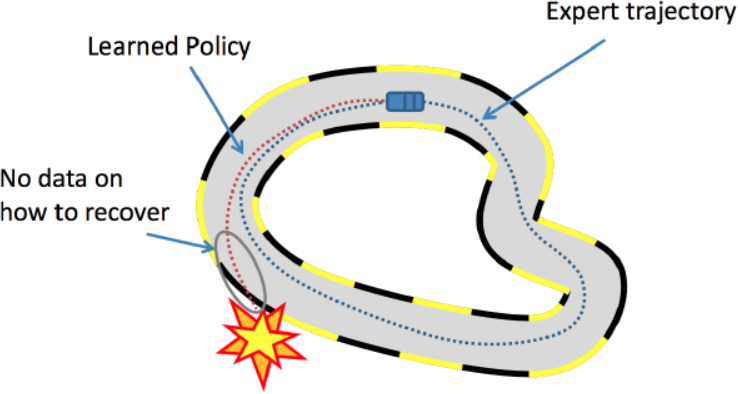
\includegraphics[width=0.35\textwidth]{Images/behavioralclonning.png}
\vspace{-0.5cm}
\end{wrapfigure}

Однако, подобная <<дистилляция знаний>> одного актёра в другого не учитывает то, что мы работаем с последовательным принятием решений. Как только наша стратегия чуть-чуть отклонится от экспертного поведения (а это, так или иначе, неизбежно) или просто получит необычный отклик от среды, она может оказаться в той области пространства состояний, где эксперта никогда не было, и примеров правильного поведения в обучающей выборке не встречалось. В такой момент клонированное поведение может выдать сколько угодно безумные результаты.

\begin{remark}
Так или иначе, клонирование поведение может сыграть роль отличной инициализации, существенно ускоряющей процесс обучения. Если для off-policy обучения имеет смысл просто докинуть экспертные траектории в буфер, то для on-policy алгоритмов при наличии экспертных траекторий имеет смысл предобучить стратегию при помощи клонирования поведения. 
\end{remark}

Во многих задачах можно побороться с этой проблемой при помощи более <<тщательного>> или <<хитрого>> процесса сбора данных; например, специально закатываясь в те области MDP, куда может заехать <<сломанная>> стратегия.

\begin{example}[DAgger]
Одна из универсальных идей звучит так: после клонирования поведения запустить полученную стратегию в среду, собрать набор тот состояний, которые она посетила, и попросить эксперта <<разметить>> их: выбрать оптимальные действия. Но такой алгоритм предполагает, что у нас есть подобное <<средство разметки>>, за счёт которого задача и сводится к обучению с учителем.
\end{example}

% TODO: пример с дроном в лесу.

\subsection{Обратное обучение с подкреплением (Inverse RL)}\label{subsec_irl}

Почему клонирование поведения --- неидеальное решение? На самом деле в разных областях пространства состояний у наших решений различается <<критичность>>: если мы ошибёмся в одном месте, наше будущее поменяется не так сильно, и эксперт в таких областях сам может выбирать довольно разнообразные действия, а в других местах от нашего решения существенно зависит дальнейшая награда, и в них крайне важно безошибочно выбрать то же действие, что и эксперт. Это означает, что функция награды как обучающий сигнал более информативен. Но зачастую функция награды нам напрямую недоступна. 

\begin{definition}
Задачей \emph{обратного обучения с подкреплением} (inverse reinforcement learning, IRL) называется задача по набору траекторий $(\Traj)$ оптимального агента восстановить функцию награды, которую он максимизирует.
\end{definition}

За счёт обратного обучения с подкреплением можно попытаться получить функцию награды, которая позволит обучить при помощи всего арсенала RL алгоритмов куда более близкую к оптимальной стратегию, чем простое клонирование поведения. Однако понятно, что задача обратного обучения с подкреплением <<некорректна>> в том смысле, что допускает всякие дурацкие решения: например, $r(s, a) \HM= 0$ всегда <<подходит>> в качестве ответа. Какой критерий качества в этой задаче, то есть как понять, насколько адекватна придуманная функция награды?

\begin{example}
Рассмотрим клеточный мир, в котором агент может ходить вправо-влево-вниз-вверх. Допустим для простоты, мы также знаем, что функция награды --- детерминированная, зависит только от состояний, и на клетках одного цвета её значения совпадают. Что мы тогда можем о ней, имея на руках одну экспертную траекторию, порождённую оптимальной стратегией?
\begin{center}
    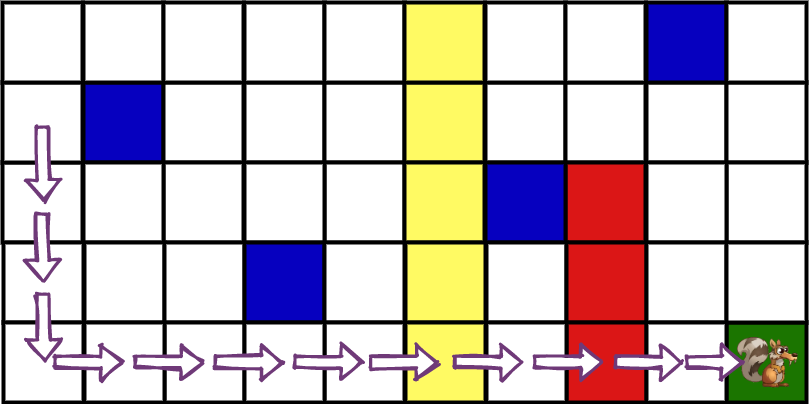
\includegraphics[width=0.7\textwidth]{Images/IRL.png}
\end{center}
На самом деле, не так много. Агент, видимо, стремился в зелёную клетку; наверное, за неё полагается положительная награда. Через красную клетку агент прошёл, хотя мог бы обойти за счёт более позднего попадания в зелёную клетку; видимо, это того не стоило, и за красную клетку награда, если и отрицательная, то совсем маленькая. Могла ли она быть положительной? Тогда бы эксперт, наверное, походил бы по красным клеткам; видимо, награда за зелёную сильно выгоднее. Синие клетки агент избегал; видимо, они или дают штраф, или ноль, поскольку если бы они давали бонус, то было бы выгодно добираться до зелёной клетки-цели через них. Наконец, про жёлтые клетки сказать почти ничего нельзя: агенту пришлось бы в любом случае пройти через них, чтобы добраться до зелёной клетки, и поэтому в них может быть как штраф (но не очень большой), так и бонус (но тоже не очень большой).
\end{example}

Ещё одна проблема задачи в том, что эксперт, обычно, не является абсолютно оптимальным. Люди не перемещаются по комнате до целей по строго прямой линии, а ходы шахматного эксперта не являются абсолютной истиной оптимальных действий.

Для упрощения формул будем везде далее полагать $\gamma \HM= 1$. Введём следующее предположение: оптимальная стратегия $\pi^*$ стохастична и генерирует такие траектории, что:
\begin{equation}\label{meirl}
p(\Traj \mid \pi^*) \propto e^{R(\Traj)} \prod_{t \ge 0}p(s_{t+1} \mid s_t, a_t)
\end{equation}

Иначе говоря, вероятность оптимальной стратегии сгенерировать ту или иную траекторию пропорциональна суммарной кумулятивной награде. Мы считаем, что стратегия эксперта, сгенерировавшего для нас датасет, удовлетворяет этому предположению. Такое предположение позволяет нам записать правдоподобие траекторий: насколько вероятно увидеть траекторию $\Traj$, если она пришла из оптимального эксперта, максимизировавшего награду в терминах \eqref{meirl}.

Откуда это предположение свалилось? На самом деле, это уже знакомый нам Maximum Entropy RL. Действительно: рассмотрим задачу поиска стратегии, которая порождает траектории из распределения \eqref{meirl}:
\begin{equation}\label{meirl_kl}
    \KL(p(\Traj \mid \pi) \parallel p(\Traj \mid \pi^*)) \to \min_{\pi}
\end{equation}

\begin{theorem}
Задача \eqref{meirl_kl} эквивалентна задаче Maximum Entropy RL \eqref{merl}.
\begin{proof}
Распишем \eqref{meirl_kl}:
\begin{align}
    \KL(p(\Traj \mid \pi) \parallel p(\Traj \mid \pi^*)) &= \E_{\Traj \sim \pi} \overbrace{\sum_{t \ge 0} \log \pi(a_t \mid s_t) + \log p(s_{t+1} \mid s_t, a_t)}^{\text{$\log p(\Traj \mid \pi)$}} - \\ &- \E_{\Traj \sim \pi} \underbrace{\sum_{t \ge 0} \log p(s_{t+1} \mid s_t, a_t) - r_t - \const(\pi)}_{\text{$\log p(\Traj \mid \pi^*)$ из \eqref{meirl}}},
\end{align}
где $\const(\pi)$ --- нормировочная константа распределения \eqref{meirl}. Убирая сокращающиеся логарифмы вероятностей переходов и домножая на минус единицу, получаем:
$$\E_{\Traj \sim \pi} \sum_{t \ge 0} \left[ r_t - \log \pi(a_t \mid s_t) \right] \to \max_{\pi},$$
что есть в точности Maximum Entropy RL.
\end{proof}
\end{theorem}

\subsection{Cost-guided Learning}

Аппроксимируем функцию награды нейросетью $r_\theta(s, a)$. Тогда правдоподобие одной траектории в предположении \eqref{meirl} равно:
$$p_\theta(\Traj \mid \pi^*) = \frac{e^{R_{\theta}(\Traj)} \prod\limits_{t \ge 0}p(s_{t+1} \mid s_t, a_t)}{Z(\theta)}$$
где $R_{\theta}(\Traj) \coloneqq \sum\limits_{s, a \in \Traj} r_{\theta}(s, a)$ --- текущая аппроксимация кумулятивной награды, а нормировочная константа, внимание, зависит от параметров нейросети $\theta$:

\begin{equation}\label{irl_partionfunction}
Z(\theta) \coloneqq \int\limits_{\Traj} e^{R_{\theta}(\Traj)} \prod_{t \ge 0}p(s_{t+1} \mid s_t, a_t) \diff \Traj
\end{equation}

Рассмотрим логарифм правдоподобия:
\begin{equation}\label{irl_loglikelihood}
\log p_\theta(\Traj \mid \pi^*) = R_{\theta}(\Traj) + \underbrace{\sum_{t \ge 0} \log p(s_{t+1} \mid s_t, a_t)}_{\const(\theta)} - \log Z(\theta)
\end{equation}

Максимизация логарифма правдоподобия имеет интересную интерпретацию: нам нужно выдавать большую награду на тех состояниях, которые эксперт посетил (первое слагаемое) и маленькую награду <<всюду в остальных местах>> (второе слагаемое). Тогда интеграл $\log Z(\theta)$ будет уменьшаться.

Как оптимизировать это правдоподобие? С первым слагаемым всё понятно: награда, моделируемая нейросеткой, дифференцируема по параметрам. Проблема заключается в нормировочном слагаемом.

Нам понадобится следующий фокус. Пусть у нас есть некоторая функция награды с параметрами $\theta$. Пусть $\pi^*_{[\theta]}$ --- стратегия, которая оптимально (в терминах Maximum Entropy фреймворка, в рамках предположения \eqref{meirl}) оптимизирует вот эту награду, которую мы предлагаем с текущими параметрами $\theta$. Такая стратегия по определению будет в среде генерировать траектории из распределения
\begin{equation}\label{irl_currentoptimalpolicy}
p(\Traj \mid \pi^*_{[\theta]}) \coloneqq \frac{e^{R_{\theta}(\Traj)} \prod\limits_{t \ge 0}p(s_{t+1} \mid s_t, a_t)}{Z(\theta)}
\end{equation}
и это в точности есть правдоподобие траекторий эксперта при текущих значениях параметров $\theta$.

\begin{theorem}[Cost-guided Learning]
Градиент для оптимизации правдоподобия \eqref{irl_loglikelihood} траекторий эксперта по параметрам функции награды $\theta$ равен:
\begin{equation}\label{costguidedlearning}
    \E_{\Traj \sim \pi^*} \nabla_{\theta} R_{\theta}(\Traj) - \E_{\Traj \sim \pi^*_{[\theta]}} \nabla_{\theta} R_{\theta}(\Traj)
\end{equation}
\beginproof
Рассмотрим градиент логарифма правдоподобия одной траектории:
$$\nabla \log p_\theta(\Traj \mid \pi^*) = \nabla R_{\theta}(\Traj) - \nabla \log Z(\theta)$$

Мы хотим оптимизировать правдоподобие в среднем по траекториям эксперта, однако нам нужен градиент нормировочной константы (общий для всех траекторий эксперта, поэтому из мат.ожидания по ним эту константу можно вынести). Рассмотрим дифференцирование нормировочной константы отдельно:
\begin{align*}
\nabla \log Z(\theta) &= \\
= \{ \text{градиент логарифма} \} &= \frac{1}{Z(\theta)} \nabla Z(\theta) = \\
= \{ \text{определение $Z(\theta)$ \eqref{irl_partionfunction}} \} &= \frac{1}{Z(\theta)} \int\limits_{\Traj} \nabla_{\theta} e^{R_{\theta}(\Traj)} \prod_{t \ge 0}p(s_{t+1} \mid s_t, a_t) \diff \Traj = \\
= \{ \text{дифференцируем экспоненту} \} &= \frac{1}{Z(\theta)} \int\limits_{\Traj} e^{R_{\theta}(\Traj)} \prod_{t \ge 0}p(s_{t+1} \mid s_t, a_t) \nabla_{\theta} R_{\theta}(\Traj) \diff \Traj = \\
= \{ \text{определение $\pi^*_{[\theta]}$ \eqref{irl_currentoptimalpolicy} } \} &= \E_{\Traj \sim p(\Traj \mid \pi^*_{[\theta]})} \nabla R_{\theta}(\Traj)    \tagqed
\end{align*}
\end{theorem}

Отсюда напрашивается такая забавная идея. С первым мат.ожиданием в формуле градиента всё понятно: мы максимизируем награду в тех парах состояние-действие, которые встречались у эксперта. Затем мы берём и при помощи любого алгоритма Maximum Entropy RL оптимизируем нашу текущую награду $r_\theta(s, a)$, получая оптимальную относительно нашей текущей функции награды стратегию $\pi^*_{[\theta]}$ (точнее, её некоторое приближение). Отправляем её в реальную среду и собираем траектории $\Traj \sim \pi^*_{[\theta]}$. И чтобы получить второе слагаемое градиента, говорим, что в состояниях-действиях, которые встретились в траекториях этого <<псевдо-эксперта>>, награду нужно минимизировать. Если наша награда стала настоящей, псевдо-эксперт сойдётся к эксперту, и градиент станет нулевым.

Конечно, мы не будем обучать RL-алгоритм для оптимизации стратегии $\pi^*_{[\theta]}$ до сходимости, и вместо этого будем чередовать шаг оптимизации по параметрам $\theta$ функции награды при помощи формулы \eqref{costguidedlearning} (где второе мат.ожидание оценено при помощи сэмплов из текущей $\pi^*_{[\theta]}$) и шаг оптимизации параметров самой $\pi^*_{[\theta]}$ при помощи RL-алгоритма. В пределе мы потенциально сойдёмся к той функции награды, которой пользовался истинный эксперт, и заодно к стратегии, её максимизирующей.

\subsection{Generative Adversarial Imitation Learning (GAIL)}

Cost-guided learning со своим чередованием двух шагов оптимизации напоминает игру двух игроков. Оптимизация по параметрам награды говорит уменьшать слагаемое, соответствующее нормировочной константе, а оптимизация стратегии --- увеличивать. У этого есть важная интерпретация, которая помогает понять, как на самом деле нужно обучаться с экспертных траекторий.

Сначала мы чуть-чуть перепишем нашу задачу оптимизации по $\pi$ и по $r$.

\begin{proposition}
Оптимизация функции награды по формуле \eqref{costguidedlearning} соответствует оптимизации следующего функционала:
\begin{equation}\label{irl_dual}
\E_{\Traj \sim \pi^*} R(\Traj) - \max_{\pi} \E_{\Traj \sim \pi} \sum_{t \ge 0} \left( r(s_t, a_t) + \entropy(\pi(\cdot \mid s_t)) \right) \to \max_{r}
\end{equation}
\begin{proof}[Пояснение]
Градиент максимума от функции есть градиент этой функции в точке максимума, а энтропия $\entropy(\pi(\cdot \mid s_t))$ не зависит от $\theta$, поэтому градиент второго слагаемого совпадает со вторым слагаемым \eqref{costguidedlearning}.
\end{proof}
\end{proposition}

\begin{definition}
\emph{Occupancy measure} для стратегии $\pi$ будем называть
\begin{equation}\label{occupancymeasure}
\rho_\pi(s, a) \coloneqq \pi(a \mid s)d_{\pi}(s),
\end{equation}
где $d_\pi(s)$ --- частоты посещения состояний \eqref{svd}.
\end{definition}

По определению, мат.ожидания по траектории с таким обозначением можно записывать как
$$\E_{\Traj \sim \pi} \sum_{t \ge 0} f(s_t, a_t) = \E_{\rho_{\pi}} f(s, a)$$

Давайте воспользуемся этим обозначением в \eqref{irl_dual}. Раскрывая определение мат.ожидания и переписывая оптимизацию по $\pi$ как минимизацию, получаем такую <<игру>> (читать --- поиск седловой точки):
\begin{equation}\label{game_pi_r}
\max\limits_{r} \min\limits_{\pi} \int\limits_{\St} \int\limits_{\A} \left(\rho_{\pi^*}(s, a) - \rho_\pi(s, a)\right) r(s, a) \diff s \diff a - \E_{\Traj \sim \pi} \sum_{t \ge 0} \entropy(\pi(\cdot \mid s_t))
\end{equation}

Сразу сделаем одно наблюдение: по определению occupancy measure однозначно задаёт стратегию $\pi$:

\begin{proposition}
\begin{equation}\label{policy_from_om}
\pi(a \mid s) = \frac{\rho_\pi(s, a)}{\int\limits_{\A} \rho_\pi(s, a) \diff a}
\end{equation}
\end{proposition}

Значит, можно вместо стратегии искать occupancy measure: действительно, в \eqref{game_pi_r} последнее слагаемое --- энтропийный бонус стратегии $\pi$ --- тоже можно переписать в терминах $\rho_\pi(s, a)$: обозначим его как
$$\tilde{\entropy}(\rho_\pi) \coloneqq \E_{\Traj \sim \pi} \sum_{t \ge 0} \entropy(\pi(\cdot \mid s_t)) = \E_{\rho_\pi} -\log \pi(a \mid s) = \{ \text{\eqref{policy_from_om}} \} = \E_{\rho_\pi} -\log \frac{\rho_\pi(s, a)}{\int\limits_{\A} \rho_\pi(s, a) \diff a}$$

Получаем такой взгляд на процесс обучения:
\begin{equation}\label{game_pi_rho}
\max\limits_{r} \min\limits_{\rho_\pi} \int\limits_{\St} \int\limits_{\A} \left(\rho_{\pi^*}(s, a) - \rho_\pi(s, a)\right) r(s, a) \diff s \diff a - \tilde{\entropy}(\rho_p)
\end{equation}

На энтропийное слагаемое $\tilde{\entropy}(\rho_p)$ можно смотреть как на регуляризатор по частотам посещения состояний. Далее мы сделаем важный шаг: мы добавим регуляризатор и для оптимизации по $r$. Во-первых, это мотивировано тем, что, как мы обсуждали ранее, задача обратного обучения с подкреплением <<некорректна>> и может иметь много разных решений. 

Есть и более важная вторая мотивация: глядя на \eqref{game_pi_rho}, видно, что единственная возможная седловая точка --- это случай $\rho_{\pi} \equiv \rho_{\pi^*}$ (как только в какой-то паре $s, a$ это не так, функция награды может начать выдавать бесконечно большие значения соответствующего знака). То есть, минимизация по $\rho_\pi$ с точностью до энтропийного регуляризатора --- это поиск такого $\rho_\pi(s, a)$, который наиболее похож на $\rho_{\pi^*}(s, a)$. Другими словами: задача обучения по экспертным траекториям заключается не в том, чтобы матчить вашу стратегию со стратегией эксперта, а в том, чтобы заматчить occupancy measure --- частоты посещений пар состояние-действие. Это сильно разные вещи: выбор одних действий в одной области пространства состояний влияет на occupancy measure в других!

Это рассуждение открывает следующую идею: давайте при обучении награды мы будем напрямую пытаться отличать распределения $\rho_{\pi^*}(s, a)$ и $\rho_{\pi}(s, a)$. Как различать распределения? Вспоминаем генеративно-состязательные сети (GAN). Там дискриминатор неявно учил различать, приходят ли сэмплы из одного класса или из другого, просто решая задачу бинарной классификации. Оказывается, это и соответствует просто определённому выбору регуляризатора!

Итак, добавим некоторое слагаемое $\psi(r)$, которое будет смотреть на нашу выдаваемую функцию награды и некоторым образом её дополнительно штрафовать:

\begin{equation}\label{game_pi_rho_reg}
\max\limits_{r} \min\limits_{\rho_\pi} \psi(r) + \int\limits_{\St} \int\limits_{\A} \left(\rho_{\pi^*}(s, a) - \rho_\pi(s, a)\right) r(s, a) \diff s \diff a - \tilde{\entropy}(\rho_\pi)
\end{equation}

\begin{theorem}
Выберем в \eqref{game_pi_rho_reg} следующий регуляризатор:
\begin{equation}\label{gail_reg}
\psi(r) \coloneqq \E_{\rho_{\pi^*}(s, a)} -r(s, a) - \log (1 - e^{-r(s, a)}),
\end{equation}
где штраф полагается бесконечно большим, если $r(s, a) \HM< 0$. Тогда задача \eqref{game_pi_rho_reg} примет вид:
\begin{equation}\label{GAIL}
\max\limits_{D} \min\limits_{\pi} \E_{\rho_{\pi^*}} \log (1 - D(s, a)) + \E_{\rho_{\pi}} \log D(s, a) + \tilde{\entropy}(\rho_\pi),
\end{equation}
где $D(s, a) \in (0, 1)$.

\beginproof
Перепишем задачу в терминах мат.ожиданий и подставим выбранный регуляризатор:
\begin{align*}
&\, \min\limits_{r} \max\limits_{\pi} \psi(r) + \E_{\rho_{\pi^*}(s, a)} r(s, a) - \E_{\rho_\pi} r(s, a) - \tilde{\entropy}(\rho_\pi) = \\
&= \max\limits_{r} \min\limits_{\pi} \E_{\rho_{\pi^*}(s, a)} \log (1 - e^{-r(s, a)}) + \E_{\rho_\pi} r(s, a) + \tilde{\entropy}(\rho_\pi)
\end{align*}

Сделаем замену переменных: вместо оптимизации по $r(s, a)$ будем оптимизировать по $D(s, a)$, где $D(s, a) \HM \coloneqq e^{-r(s, a)}$ --- произвольное число в диапазоне (0, 1). Тогда $r(s, a) = -\log(D(s, a))$.
\begin{equation*}
\max\limits_{D} \min\limits_{\pi} \E_{\rho_{\pi^*}(s, a)} \log (1 - D(s, a)) + \E_{\rho_\pi} \log D(s, a) + \tilde{\entropy}(\rho_\pi)   \tagqed
\end{equation*}
\end{theorem}

Итак, что мы получили в формуле \eqref{GAIL}: вместо награды будем обучать дискриминатор, решающий задачу бинарной классификации, где пары $s, a$ из $\rho_{\pi^*}$ образуют класс 1, а пары $s, a$ из $\rho_\pi$ --- класс 0. Действительно, оптимизация \eqref{GAIL} по $D$ при фиксированной $\pi$ выглядит так:
$$\E_{\rho_{\pi^*}} \log (1 - D(s, a)) + \E_{\rho_{\pi}} \log D(s, a) \to \max\limits_{D},$$
то есть мы просто учимся отличать пары $s, a$, порождённые (встреченные) экспертом от тех, что встречает наша текущая стратегия. 

Оптимизация же по $\pi$ (давайте вернёмся к оптимизации по стратегии) при фиксированном <<дискриминаторе>> $D$ выглядит так:
$$
\E_{\Traj \sim \pi} \sum_{t \ge 0} \left[ -\log D(s_t, a_t) + \entropy(\pi(\cdot \mid s_t)) \right] \to \max\limits_{\pi}
$$
То есть величина $-\log D(s, a)$ и будет являться наградой за шаг: именно такую кумулятивную дисконтированную награду (плюс энтропийный бонус) оптимизирует стратегия $\pi$, она же <<генератор>> в этой схеме.